
\section{Lecture 7: Weight, perceived gravity, and weightlessness}

This lecture will discuss weight, its relation to mass, and other related topics.

A regular scale, say a bathroom scale, measures weight -- which is a \emph{force}.
The force of the scale is $F_s=mg$, the scale uses the gravitational constant of earth $g$.
Thus, there is only one unknown $m$, which can be derived from $m=\frac{F_s}{g}$.

If we were to use the same scale on the moon, which has a mass of $1/6$ of earth, the 
scale would show that your mass is $1/6$ of what it is since it uses $g$ of earth.

Now, we move the scale and you into an elevator.

\begin{figure}[H]
  \centering
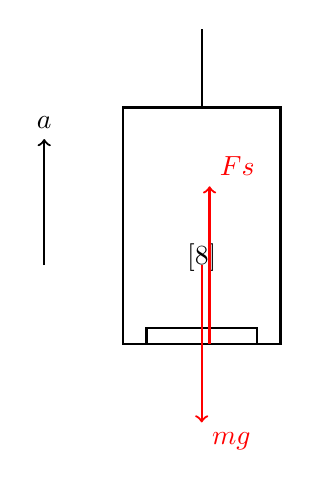
\begin{tikzpicture}
  \pgfmathsetmacro{\ax}{1}
  \pgfmathsetmacro{\ay}{0}
  \pgfmathsetmacro{\bx}{\ax + 2}
  \pgfmathsetmacro{\by}{\ay + 3}
  \pgfmathsetmacro{\cx}{\ax + 1}
  \pgfmathsetmacro{\cy}{\ay+1.1}
  \pgfmathsetmacro{\ddx}{\bx-\ax}
  \pgfmathsetmacro{\dx}{\ax + \ddx/2}

  \draw[thick] (\dx, \by) -- (\dx, \by+1);
  \draw[thick] (\ax, \ay) rectangle (\bx, \by);
  \draw[thick] (\ax+0.3, \ay) rectangle (\bx-0.3, \ay+0.2); % Scale
  \node at (\cx, \cy) {\Strichmaxerl[8]};

  \draw[thick, ->] (0, 1) -- (0, 2.6) node[above] {$a$};
  \draw[thick, red, ->] (\dx+0.1, \ay) -- (\dx+0.1, \ay + 2) node[above right] {$Fs$};
  \draw[thick, red, ->] (\dx, \ay+1) -- (\dx, \ay-1) node[below right] {$mg$};
\end{tikzpicture}
\end{figure}

Again, gravity acts on you with a force $m g$ downwards. The scale pushes back up with force $F_S$. However, now, the elevator is being accelerated upwards. The net force must now be positive (upwards), not zero, since you could not have a nonzero acceleration with zero net force.

We find that $F_S - m g = m a$, so $F_S = m(a + g)$. The reading of the scale has increased, and increases linearly with increasing acceleration upwards. If the elevator accelerates upwards at $2g \approx \SI{20}{m/s^2}$, your weight would be three times as high as usual. Only when $a_y = 0$ is your measured weight as it usually is.

Let's now reverse the situation. We now consider increasing $a$ to be downwards, and the elevator is now accelerating downwards. In other words, $a > 0$.

Again, you have gravity acting downwards with a magnitude $m g$. If that were the only force, you would be in free fall with acceleration $g$, so there must be some upwards acting force. On the other hand, $|m g| > |F_S|$ or there would be no acceleration at all, so while $|F_S|$ is smaller than the force gravity exerts on you, it's still there.

Back to Newton's second law.

\begin{equation}
m g - F_S = m a
\end{equation}

Reading that out loud, it does make a lot of sense: if $F_S = m g$, then $m a$ is zero, and we are not accelerating. If $m g$ is dominant, we are accelerating downwards (since $a > 0$ means downwards acceleration).

Rearranged,

\begin{equation}
F_S = m(g - a)
\end{equation}

The larger the downwards acceleration, the \emph{less} you weigh. I think most of us have experienced this (and the reverse situation) in fast elevators (that accelerate quickly).

Now, imagine we cut the cable of the elevator. What happens? Well, our equation has the answer. The net acceleration $a$ will be equal to the acceleration from gravity $g$, so $F_S = 0$. That is, the scale will show you to have zero weight -- and you will, because you are now in free fall. You are falling downwards, but other than that, you wouldn't notice gravity the same way we do now. The things falling with you wouldn't care about up or down -- a glass filled with water would act the same whether upside down or not.

This is very similar to how things work in the space shuttle and on the International Space Station (ISS). Their orbits around the Earth keep them in constant free fall, only they never hit the surface, as they are going sideways with great velocity (about 7.7 km/s!). We will talk much more about orbits later in the course.

In short, weightlessness is when the forces acting on you are exclusively gravitational. You're not being held up by any floors, ropes, seats, etc, just falling due to gravity pulling on you.

Let's now look at another type of scale:

\begin{figure}[H]
  \centering
\begin{tikzpicture}[scale=1]

  \draw[thick] (0,2) circle (8pt);
  \node at (0,0) {\Strichmaxerl[7]};
  \draw[thick] (0,1.8) -- (0,0.9);
  \draw[thick] (0.4,0.0) -- (0,1.5);
  \draw[thick] (-0.4,0.0) -- (0,1.5);
  \draw[thick] (-0.4,0.0) -- (0,1.5);

  \draw[thick, red, -{Stealth[scale=1.5]}] (0,0.1) -- (0,2) node[midway, right = 2mm] {$T=mg$};
  \draw[thick, red, -{Stealth[scale=1.5]}] (0,-0.1) -- (0,-2) node[midway, right = 2mm] {$mg$};

\end{tikzpicture}
\end{figure}

The scale in this case is a tension meter, inside the string we are hanging from. Because we are hanging still, not accelerating, the tension in the string must equal the force of gravity pulling us down. Therefore, the tension meter reads $m g$, same as it would on a regular scale standing on the floor.\\
Thus, we see that it makes no difference whether we measure the force a scale is pushing us up with, or the force a rope/tension meter \emph{pulls} us up with.

Let's now accelerate this system. We accelerate it upwards, which must mean the tension in the string goes up -- it must be greater in magnitude than $m g$ or we wouldn't accelerate upwards.\\
Just as with the elevator, we find $T - m g = m a$ or $T = m(a + g)$. Same as before, only we use $T$ for tension instead of $F_S$ for force exerted by the scale.\\
If we instead accelerate downwards, we again find the same result as before, as do we if we simply cut the string and go into free fall.

Say we have the following system:

\begin{figure}[H]
  \centering
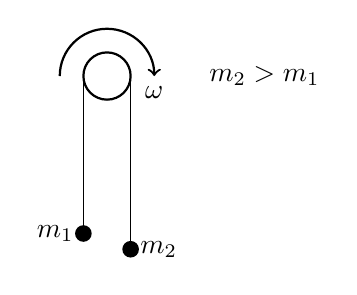
\begin{tikzpicture}[scale=1]

  \draw[thick] (0,2) circle (3mm);
  \fill[thick] (-0.3,0) circle (3pt);
  \fill[thick] (0.3,-0.2) circle (3pt);

  \draw (-0.3,2) -- (-0.3,0) node[left] {$m_1$};
  \draw (0.3,2) -- (0.3,-0.2) node[right] {$m_2$};

  \node at (2,2) {$m_2>m_1$};

  \draw[thick, ->] (-0.6,2) arc[start angle=180, end angle=0, radius=6mm] node[below] {$\omega$};

\end{tikzpicture}
\end{figure}


The string is massless, the pin/pulley is massless, but the two objects hanging an each end are not; the right one at mass $m_2$ has a greater mass than that of $m_1$ to the left.

What happens? Well, we know from intuition and experience that the system will accelerate as shown. $m_2$ will fall down, while $m_1$ will be pulled up.

Because we consider the case where there is no friction, and the string is massless, the tension in the left side must equal the tension on the right side. Only in the case of no friction and a massless string is this true, however.

Why is that, though? It's relatively easy to show. Consider a small piece of the string on the left side. It has gravity pulling the mass $m_1$ down, and a force upwards because of the mass $m_2$ on the other side of the pulley. If the two forces were not equivalent, the massless string would experience an acceleration $a = \frac{F}{0}$ -- that's clearly impossible.	

The same argument can be used for any part (of any length) of the string. The tension must be equal everywhere.\\
Again, this is only true because we consider the string massless, and the pulley frictionless.

Now, we earlier showed that the tension in the string is an indicator of the weight hanging from it. That means that while this acceleration is taking place, $m_1$ and $m_2$ have the same weight! The obviously don't have the same \emph{mass}; that's different, by definition of $m_2 > m_1$. Because weight is mass times acceleration, however, the \emph{weight} of $m_1$ has increased, as it is being accelerated upwards (think about the elevator and the bathroom scale), while the weight of $m_2$ has \emph{decreased}, since it is accelerating downwards (falling, though not in free fall, so it still has a weight larger than zero).

Let's calculate the acceleration and tension for these objects and strings.\\
$m_1$ accelerates upwards. The tension in the string is $T = m_1 g$ while it is in equilibrium, but that cannot be the case now. The force upwards must be greater than $m g$, or it cannot accelerate upwards. Therefore, the tension in the string must be the sum of the downwards force due to gravity, plus the extra ``perceived'' gravity from the upwards acceleration. In total, we have $T = m_1 a + m_1 g = m_1(a + g)$.

For the second object, gravity pulls downwards with force $m_2 g$, while the string tension pulls back up. This object is accelerating downwards, however, so $m_2 g$ must be greater in magnitude than the tension. However, remember that the tension must be the same as in the case of the first mass! It's the same string, and as we showed earlier, we get an impossible situation if the tension differs throughout the string.

To avoid sign confusion, we now denote \emph{downwards} acceleration to be positive. We write the tension out as an equation, and find $T = m_2 (g - a)$.

We now have two equations, so we can set them equal and solve for the acceleration $a$:

\begin{align}
T = m_1(a + g)\\
T = m_2(g - a)\\
m_1 a + m_1 g = m_2 g - m_2 a\\
m_1 a + m_2 a = m_2 g - m_1 g\\
a(m_1 + m_2) = g(m_2 - m_1)\\
a = \frac{g(m_2 - m_1)}{m_1 + m_2}\\
\end{align}

We can then substitute that value into $T - m_1 g = m_1 a$ that we found earlier:

\begin{align}
T - m_1 g = m_1  \frac{g(m_2 - m_1)}{m_1 + m_2}\\
T = \frac{2 g m_1 m_2}{m_1 + m_2}
\end{align}

The algebra isn't shown, but this is indeed the case.\\
These two results make intuitive sense. If we set $m_1 = m_2 = m$, we find $T = m g$ and $a = 0$. All is as it should: the tension on a string with a weight $m$ hanging from it better be $m g$, if it's not accelerating! Likewise, $a$ better be zero, since both masses and weights are equal, so there is no net force on either mass.

If we even consider as $m_2 \to 0$, we find that the tension goes to zero, and the acceleration goes to $g$ (in magnitude). This is because $m_1$ is now in free fall, and since $m_2$ is massless and the string is massless, there is nothing left to cause tension in the string. The acceleration is $-g$ since it is simply in free fall -- nothing is holding it up.

We can also show that if $m_2 > m_1$, then the relationship $m_1 g < T < m_2 g$ will hold for this system. As they are being accelerated, the tension will be equal for both masses. Therefore, $m_1$ must gain weight, and $m_2$ must lose weight. (Keep in mind that $m_1$ accelerates upwards, so it gains weight, like in an elevator, and $m_2$ accelerates downwards, and so it loses weight.)

\subsection{Weightlessness}

We talked a bit about perceived gravity and so on last week. Let's expand on it.

Consider the case where we are swinging an object around a rope of length $R$ in the vertical plane. $R$ is then the radius of the circle the object traces out.\\
Gravity with force $m g$ acts downwards at all times. We spin the object with angular velocity $\omega$.

The string will have a tension $T$, which will change in direction as the thing spins, of course. The magnitude should also change -- if the angular velocity is low, just on the edge of this working out, the tension should be zero at the top. Any slower, and the string will slack off and the object starts falling down.

Let's calculate the tension. First, we know there will be a centripetal acceleration $|a_c| = \omega^2 R$. That must be the case, or the object cannot travel around in a circle like this, period.

At the lowest point of the circle, gravity acts downwards with force $m g$, while the tension upwards is $T$. There's also the centripetal force $m a_c$. We have not really used the term centripetal force yet, but it's a force, so it's found by the centripetal acceleration times the mass in question.

All in all, we find $T - mg = m a_c$, so that $T = m(a_c + g)$. This equation looks almost exactly like the one for acceleration in an elevator, which we found earlier. If $a_c = g$, you tension of the string would be twice the weight of the object.

Now, let's look at the top of the circle instead. As we did earlier, we will now reverse out sign convention so that downwards forces and accelerations are positive.\\
As before, the tension and the force of gravity add up to the centripetal acceleration, so we find $T + m g = m a_c$, so that $T = m(a_c - g)$.

This is just about exactly the same equation as we had for the elevator accelerating downwards, losing weight.\\
If $a_c = g$, the tension will be zero, and the object will be weightless. If $a_c > g$, there will be tension in the string, equal to the object's weight.\\
$a_c$ cannot be smaller than $g$, however. That would give us negative tension, which can't happen. What this implies is that this situation simply would never happen: if $a_c < g$, then the object would never reach the top while tracing out a circle, but would have started falling prior to reaching the top.

The rest of the lecture is mostly demonstrations and related talk, which I didn't find it very useful to take notes for, but it's certainly worth watching, of course.\\
One thing is worth writing down though. The lecture talks about parabolic plane flights -- they start by upwards at a $\approx 45$ degree angle, then follow a parabolic trajectory (free fall) with the engines off, and then re-start the engines and repeat.

This causes the plane to be in free fall for about 30 seconds at a time, during which time any traveler would experience weightlessness -- but \emph{not zero gravity}. There are absolutely similarities between free fall and zero gravity (which you could almost experience far, far from any planets or stars, but certainly not on Earth), but they are not the same.

Zero gravity implies that the Earth's gravity somehow stops acting on the people in the plane, despite the fact that Earth's gravity is almost as strong up there as it is at the surface. Even at the ISS, in orbit at an altitude of about 350 km (which is quite close to the surface for a ``space'' station, all things considered), the gravitational pull is about 90\% of the strength it is near the surface.\\
The astronauts are then weightless for exactly the same reason: they are constantly falling ``towards'' the Earth, only they have such a huge sideways velocity, that they never hit it.

We will talk more about gravity later in the course, including how $g$ is calculated etc.

\section{Lecture 8: Frictional forces}

Let's talk about friction. Thus far, we have ignored friction (and air drag) in all problems we've solved; that will now start to change.

Let's look at a simple case to begin with. We have an object at rest, on a flat surface:

\begin{center}
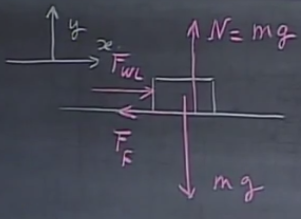
\includegraphics[scale=0.8]{\pIImages/lec8_friction}
\end{center}

There is a gravitational force of magnitude $m g$ pulling the object down, and a \emph{normal force} $N = m g$ (also in magnitude) from the surface on the object, or it could not be at rest; Newton's second law. (Again, however, note that this is NOT a case of Newton's third law; there two forces both act on the object, and so they are not an action-reaction pair.)

We (the professor) exerts a force $F_{WL}$ (WL for Walter Lewin) in the $+x$ direction. Because of friction, the object will not start to move unless the force is great enough. (Without friction, any force, no matter how small, causes an acceleration, even if it's tiny.)

There is a frictional force $F_F$ in the $-x$ direction that exactly cancels out the force we apply. We push harder and harder, and eventually the frictional force reaches its maximum value, at which point we overcome it and the object starts to accelerate.

It is then experimental fact that this maximum, $F_{Fmax}$, is

\begin{equation}
F_{Fmax} = \mu N
\end{equation}

where $\mu$ is a friction coefficient.\\
We can differentiate between the \emph{static} friction coefficient $\mu_s$ and the \emph{kinetic} (or dynamic) friction coefficient $\mu_k$.

$\mu_s N$ is the frictional force we need to overcome to get a resting object to start moving, while $\mu_k N$ is the force we need to overcome to keep accelerating it. (If $\mu_k N = F$, there is zero net force, and so no acceleration. If $\mu_k N > F$, the object will slow down.)\\
We know from experience that it takes more force to get something to move in the first place, so $\mu_s > \mu_k$ -- ``always'', the lecture says, but there does appear to be some strange exceptions to this rule. I'm assuming this course will not cover (or mention) them, however.

We can calculate a friction coefficient by putting an object on an incline, and measure the angle of incline required to get the object to move (due to the gravitational force downwards, of course).

\begin{center}
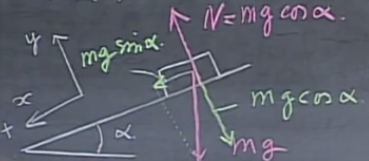
\includegraphics[scale=0.8]{\pIImages/lec8_friction_incline}
\end{center}

Note the choice of coordinate system, which is tilted such that the acceleration (and movement) in the $y$ direction will always be zero, but more importantly such that the $y$ axis is exactly perpendicular to the surface of the incline.\\
The downside to this approach is then that we need to decompose the gravitational force, since it is no longer strictly in one axis.

Because of how the angle $\alpha$ is defined, the strength of the gravitational force in the $y$ direction is $m g \cos \alpha$ (if $\alpha = 0$, $\cos \alpha = 1$ and so it is strictly in the $y$ direction), while that in the $x$ direction is $m g \sin \alpha$. This is a bit opposite to how it usually is ($x$ tends to use the cosine, while $y$ uses the sine), but it should make sense why this is.

There is a normal force $N$ opposing $m g \cos \theta$, which must be equal in magnitude -- there is no acceleration in the $y$ direction, so the net force along that axis must be zero, via Newton's second law.

There is a frictional force $F_F$ in the negative $x$ direction, equal in magnitude to $m g \sin \alpha$ (the gravitational force along the slope), since the object is still not moving. We gradually increase the angle, which increases $F_f$, but of course also the gravitational force in the $x$ direction (downwards along the slope). Sooner or later, the frictional force reaches its maximum, and gravity ``wins''.

How do we then calculate $\mu_s$, the static friction coefficient, in terms of the angle $\alpha_{max}$ (the maximum angle possible before the object starts to slide)?

Well, it should be easy! We know the strength of the force pulling the object: $m g \sin (\alpha_{max})$. We know that $F_F = \mu_s m g \sin (\alpha_{max})$ must exactly equal this force in magnitude to keep it standing still.\\
We also know that $F_F = \mu_s N$, as we mentioned earlier.

Therefore, we set the two equal, and we can solve for $\mu_s$. $N = m g \cos \alpha$, so

\begin{align}
\mu_s m g \cos (\alpha_{max}) = m g \sin(\alpha_{max})\\
\mu_s = \frac{m g \sin(\alpha_{max})}{m g \cos (\alpha_{max})}\\
\mu_s = \frac{\sin(\alpha_{max})}{\cos (\alpha_{max})} = \tan(\alpha_{max})
\end{align}

So finding the static friction coefficient is truly simple: measure the maximum angle possible before the object starts to slide, take the tangent of that angle, and you're done! And, since the incline makes a triangle with the vertical height, horizontal length and the incline itself (the hypotenuse), we can measure this even without knowing angles; we can calculate the angle even if we can only measure distances.

Note that two seemingly important quantities are nowhere to be seen in this result: the mass of the object does not matter, and neither does the amount surface area that is in contact with the incline!\\
This means that two parked cars -- a large truck and a small car,will start to slide at the same angle, if they were tilted together, so to speak. Not only does the mass not matter, but the width of the tires (or the number of tires) also does not matter.

These two facts are then demonstrated qualitatively, by sliding a few objects down a wooden plank. Indeed, adding a few times the mass to a plastic container didn't change the result by much (but by a little -- because the plank is not exactly uniform, the containers may not be identical, etc.). Neither did it make a noticeable difference to slide down two small pieces of wood, one lying down (large contact area) and one standing on the edge (small contact area).

\subsection{Friction on a block with a pulley}

Let's look at a different, but related example. We have the following setup:

\begin{center}
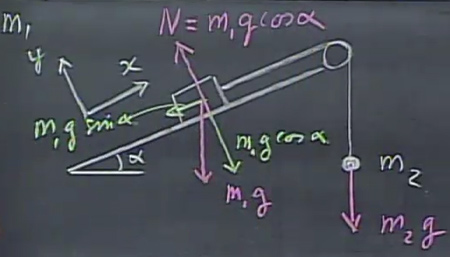
\includegraphics[scale=0.7]{\pIImages/lec8_friction_pulley}
\end{center}

A block of mass $m_1$ is sitting on an incline, with the same gravitational force, decomposed as previously.\\
However, this time, a second mass $m_2$ hangs on a massless and fixed-length string (increasing tension doesn't increase the length of the string), over a pulley (which itself is massless and frictionless).

As before, there is no movement of the  block in the $y$ direction, so we be sure that the normal force $N$ must exactly cancel out the gravitational force of $m_1 g \cos \alpha$ in our rotated $-y$ direction.\\
The string has a tension, since mass $m_2$ is hanging on it. As before, since the string is massless and has a fixed length, the tension must be the same everywhere in the string.

Now... This situation has a tricky part that the previous one didn't: depending on the friction coefficient of the block, and the magnitude of masses $m_1$ and $m_2$, one of three things can happen: the block can accelerate ``downhill'', it can accelerate ``uphill'', or it can simply stand still. We need to consider all of these possibilities when solving this problem. Because of this, we do not know in which direction of the frictional force is; we only know that it always opposes the object's motion, which could be either $+x$ or $-x$.

We do know that the maximum magnitude of the frictional force is

\begin{equation}
F_{Fmax} = \mu_s N = \mu_s m_1 g \cos \alpha
\end{equation}

The tension in the string, $T$, can be drawn as a vector opposing $m_2 g$, in the string above mass $m_2$.

We will now evaluate three different situations. In all cases, the system is at rest for now, but what is about to happen differs: there's the case where it's \emph{just} about to start accelerating towards the left (downhill for the block), the case where it's \emph{just} about to start accelerating in the other direction, and the case where it will remain at rest/in equilibrium.

Because the system is rest, the tension must be of magnitude $m_2 g$, so that it exactly balances the gravitational force on mass $m_2$, and as mentioned previously, that tension is the same in all parts of the string.

\subsubsection{Case 1: About to accelerate uphill}

We will first look at the case where $m_2$ ``wins'', and the block is \emph{just} about to start moving uphill, but is \emph{still at rest}.\\
In this case, the frictional force is at a maximum $F_{Fmax}$, which opposes the direction it's about to move it, so $F_{Fmax}$ acts together with gravity in the $-x$ direction.\\
We can write Newton's second law for the system:

\begin{equation}
T - m_1 g \sin \alpha - F_{Fmax} = 0\text{ (we substitute $T = m_2  g$)}
\end{equation}
\begin{equation}
m_2 g = m_1 g \sin \alpha + F_{Fmax}
\end{equation}

Tension acts ``uphill', while the other two act ``downhill'', and they must sum to zero since $a$ is still zero.

When this equation is true, the block is \emph{just} about to move uphill. Therefore, we can write a criterion for the uphill motion:

\begin{equation}
m_2 g \ge m_1 g \sin \alpha + F_{Fmax}
\end{equation}

If $m_2$ increases in mass by even the tiniest bit, the system will start to accelerate so that $m_2$ starts moving downwards.

\subsubsection{Case 2: About to accelerate downhill}

In this case, the frictional force is in the same direction as the tension, and thus in the opposite direction of gravity. We write Newton's second law again:

\begin{equation}
T + F_{Fmax} = m_1 g \sin \alpha\\
\end{equation}
\begin{equation}
m_2 g = m_1 g \sin \alpha - F_{Fmax}
\end{equation}

If $m_2$ is just a tiny bit \emph{smaller} (or $m_1$ greater, or $F_{Fmax}$ smaller), the system will start moving downhill. Therefore, the criterion for downhill motion is

\begin{equation}
m_2 g \le m_1 g \sin \alpha - F_{Fmax}
\end{equation}

\subsubsection{Case 3: Neither case matches}

In case neither of the two conditions are met, the system will simply sit in equilibrium. The frictional force will be ``adjusted'' so that it causes the net force in the $x$ direction to equal zero.

\subsubsection{Example case}

Let $m_1 = \SI{1}{kg}$, $m_2 = \SI{2}{kg}$, $\mu_s = 0.5$ and $\mu_k = 0.4$, while using $g = \SI{10}{m/s^2}$ for our calculations, just to get an idea. Also, let $\alpha = \ang{30}$.

What will happen in a system with these parameters? Well, we have three possible cases, with equations (or inequalities) we can look at. Since both conditions depend on the same three force terms, let's calculate their values:

\begin{align}
m_2 g &= \SI{20}{N}\\
m_1 g \sin \alpha &= \SI{5}{N}\\
F_{Fmax} = \mu_s m_1 g \cos \alpha &\approx \SI{4.33}{N}
\end{align}

Let's now look at each of the two conditions. For the block to start sliding uphill, substituting in the values, we must have $\SI{20}{N} \ge \SI{5}{N} + \SI{4.33}{N}$. Since that is true, the block will indeed start sliding uphill. Let's just verify that the second case is false, just for the sake of argument. We need $\SI{20}{N} \le \SI{5}{N} - \SI{4.33}{N}$, which is certainly not the case. So indeed, only one case matches, and it says the block will start accelerating uphill.

Let's now attempt to calculate the magnitude of the acceleration, and the string tension. We know that it will start moving uphill, so the frictional force is then downhill, in the $-x$ direction. The magnitude of this force now changes, however: the block is in motion, and so we must now use the kinetic friction coefficient $\mu_k$ instead. Using that, we find

\begin{equation}
F_{Fmax} = \mu_k m_1 g \cos \alpha
\end{equation}

We can again write Newton's second law for this case. The tension is uphill, gravity downhill, and friction downhill. Those forces must equal $m_1 a$, where $a$ is the uphill acceleration. (Since the block is now being accelerated, the net forces no longer sum to zero.)

\begin{equation}
T - m_1 g \sin \alpha - \mu_k m_1 g \cos \alpha = m_1 a
\end{equation}

We need a second equation, however. $T$ is unknown -- because $m_2$ is now being accelerated downwards, it is ``falling'' or ``losing weight'', so $m_2 g > T$ or the object could not accelerate down!\\
Since $m_2$ will never change, and we are still on Earth's surface, $g$ can also not change. The only thing that \emph{can} change is the tension. The tension \emph{must} go down, or $m_2$ simply cannot accelerate downwards!

The second equation can be found by thinking about mass $m_2$. Because the string has a fixed length, the acceleration of this mass \emph{must} be equal to that of the block sliding uphill. Anything else and clearly, the string would need to get either longer or shorter, depending on which acceleration was greater.

Because they are equal in magnitude, then, we can write a second law equation for mass $m_2$, using positive values for the downwards direction (so that this $a$ has the same positive sign as the other $a$ uphill):

\begin{equation}
m_2 g - T = m_2 a
\end{equation}

Solving this system, we get a fairly complex answer, unless we substitute in the numbers early. If we do, we find $a \approx \SI{3.85}{m/s^2}$ and $T \approx {SI}{12.3}{N}$. If we don't, we find, after simplification,

\begin{equation}
a = g\ \frac{m_2 - m_1 (\mu_k \cos \alpha + \sin \alpha)}{m_1 + m_2}
\end{equation}

And for the tension:

\begin{equation}
T = g m_1 m_2 \frac{1 + \mu_k \cos\alpha + \sin \alpha}{m_1 + m_2}
\end{equation}

Two things are important to note from the numerical results we found. One is that the acceleration was a positive number. We had already calculated that the block should move uphill, and since the positive $x$ direction is uphill, a negative acceleration would mean it should move backwards. We already know that is not the case, so the acceleration must be positive in this case.

Second, the tension must be smaller than $m_2 g$, or that mass couldn't possibly be accelerating downwards. If $m_2 g$ doesn't ``win'' over the tension, how could the mass be accelerating downwards?

Let's take a quick look at what would happen in the same system, if $m_2 = \SI{0.4}{kg}$ instead. In that case, $m_2 g = \SI{4}{N}$. Let's look at the conditions again. Is it true that $\SI{4}{N} \ge \SI{5}{N} + \SI{4.33}{N}$? No, certainly not. Is it then true that $\SI{4}{N} \le \SI{5}{N} - \SI{4.33}{N}$? No, that's not it, either.

Since neither condition is met, the system will stay as it is, with $a = 0$. Note that the equations we derived just above, for $a$ and $T$, are not valid in this case and cannot be used. They only hold in the case of accelerations upwards, since that is what we derived them for.

What will happen is that the frictional force will be adjusted so that together with the tension, it holds the object up.
